\documentclass[a4paper,10pt]{article}
\usepackage[utf8]{inputenc}
\usepackage{url}
\usepackage{amsthm, amscd, amsfonts, amssymb, graphicx,tikz, color, environ}

%opening
\title{Literature Review: Simulating Flexible Assembly System Event Logs for the Purposes of Process Modelling and Machine Learning – DRAFT}
\author{Tero Keski-Valkama}

\begin{document}

\maketitle

\smallskip
\noindent \textbf{Keywords.} Flexible Assembly System, Discrete Event Simulation, process mining, uncorrelated event streams, multi-modal representation

\section{Topic}
Flexible Assembly System is a modular and reconfigurable assembly and tooling workshop with a focus on small and medium-sized batches of varying products.
Flexible Assembly System was described formally by Donath and Graves \cite{donath1988flexible} as a system consisting of a set of products each with a specified volume
assembled on a workshop consisting of a fixed number of cells.

The assembly steps are performed in cells in parallel. Assemblies and components are transported to the cell where they are combined, tooled or inspected. Products
are transported out of the cell for the next assembly step in another cell, or out of the system as end products.
The work steps executed in the cells can be manual or automatic. There can be a central storage such as a shelf for storing components, the intermediate assemblies between the steps
and the end products waiting to be transported out of the system.

Flexible Assembly System work loads consist of small and medium sized batches where there can be some variation in the products based on customization and personalization.
The Flexible Assembly Systems are modular and often composed out of independent modules from different suppliers. The Flexible Assembly System event trace consists
of events received from all the separate modules of the system, and additional sensors and triggers added to the system in integration phase or later.

Using a Flexible Assembly System to assemble batches of products generates an electronic event trace which is logged. The events in the event trace are typically at least
partially agnostic to the assembly process being performed, and therefore the events do not include tokens connecting the event to a specific final product instance.

Simulating these kinds of event traces provides valuable material for learning systems which can be used to derive assembly process models and to detect deviances.
It is in principle possible for an automatic system to detect features in the given material in an unsupervised fashion at least when a human is capable of doing so.
A multimodal approach is convenient in data representation when we need to explore human pattern recognition capabilities. In specific, data visualization as audio
allows a human to understand the data melodies, rhythms and possible canon-like features.

\section{Description of Method}

A proper literature review is a methodological, continuous process. The goal of the literature review is to accumulate a body of relevant existing knowledge
about the topic, categorized based on subtopics and keywords.
Ultimately the literature review can be presented in the article in a summary form to present the context of the research.
The collected references represent a focused area of the existing literature relevant to the object of research.

The review starts from discovery, discovering information sources and starting points of review. The literature review process progresses towards synthesis
where the relevant existing knowledge is synthesized together to form an understanding of the composite.

The discovery phase includes a listing of subtopics and keywords, to structure the gathered discovered information into a manageable form. The goal
of the discovery phase is to form questions about the existing knowledge and to find answers to them.

The synthesis is composed of the description of the existing knowledge and possible gaps related to the research.

\section{Discovery Phase}

The topic under review is somewhat cross-discplinary relating to industrial assembly processes, business process modelling and learning systems.
Overall the following subtopics are recognized:
\begin{enumerate}
 \item Assembly process modelling and simulation
   \begin{enumerate}
     \item Fault modelling and simulation
   \end{enumerate}
 \item Mathematical analysis of log data
   \begin{enumerate}
     \item Analysing interleaved process traces
     \item Analysing delays and intervals
   \end{enumerate}
 \item Process mining
 \item Visualization of event logs
\end{enumerate}

\begin{figure}[ht]
\begin{center}
 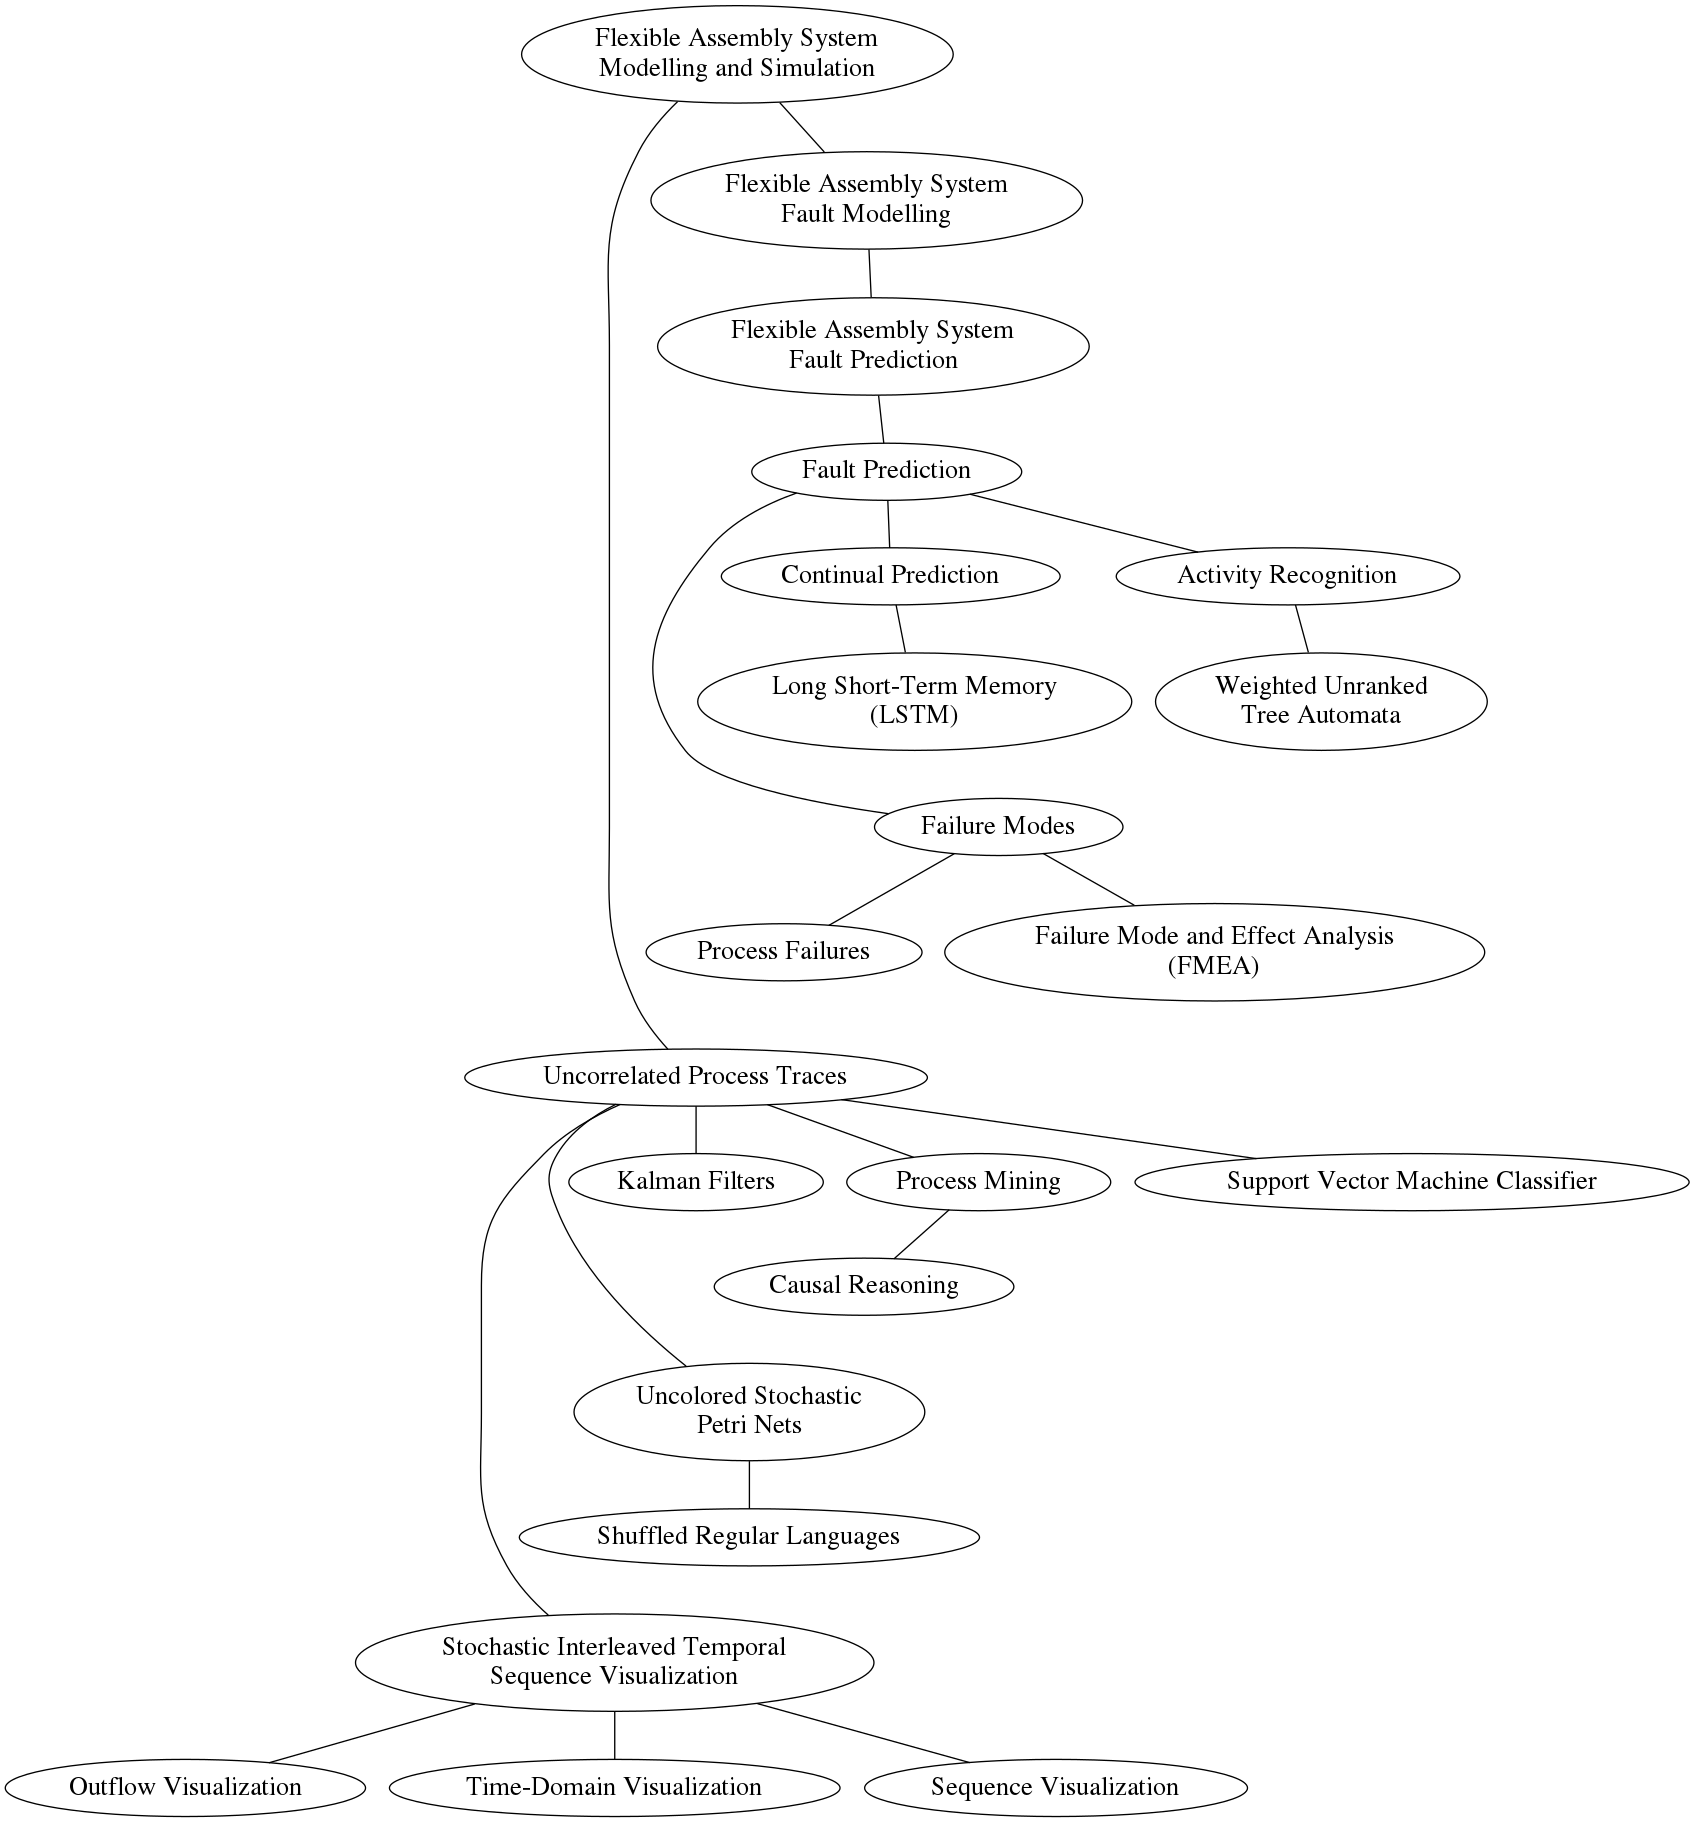
\includegraphics[width=\textwidth]{./field.png}
 % field.png: 0x0 pixel, 300dpi, 0.00x0.00 cm, bb=
\end{center}
\caption{The mind map of the research topic}
\end{figure} 

\subsection{Keywords}

The keywords relevant for the research were collected from a set of articles deemed especially relevant for this research. A representative set of articles was
read and relevant keywords were picked from titles, abstracts and references. This set of keywords allows for directed browsing of relevant literature.

\begin{itemize}
 \item assembly process
 \item assembly system
 \item complex robotic system
 \item compliant parts
 \item dimensional quality
 \item dimensional variation propagation
 \item discrete event system
 \item Failure mode and effects analysis (FMEA)
 \item failure rates
 \item failure records
 \item failure report
 \item fault detection
 \item fault mode
 \item fixture variation
 \item interleaving
 \item leaf spring
 \item multiple failure modes
 \item Multi-Station Assembly Systems
 \item outflow visualization
 \item part variation
 \item petri nets
 \item Process algebra Petri Net (PPN)
 \item process control
 \item process failures
 \item process FMEA
 \item reduction of irregularities
 \item reliability
 \item simulation
 \item sonification
 \item time-domain visualization
 \item uncolored petri nets
 \item uncorrelated event streams
 \item variation propagation
 \item visualization of sequences
 \item welding gun variation
\end{itemize}

\subsection{Core Questions}

The core questions about the existing literature are:
\begin{enumerate}
 \item How are assembly systems described and modelled?
 \item What methods are there to model and simulate assembly processes and related faults?
 \item What methods are there to visualize and represent event logs with or without timestamps?
 \item What are the relevant keywords and terms to describe this problem space?
\end{enumerate}

\section{Synthesis}

Assembly systems, construction processes and business processes are often simulated using discrete event systems, for example in:
\cite{hlupic1998business,zhao2010efficient,kang2013active,rahnama2010fuzzy}. These simulations are used for process optimization\cite{sadeghi2008framework}, scheduling and
assembly line design. The models of these systems are conveniently described using Process algebra Petri nets (PPNs) \cite{falkman2007specification}.

The literature about faults and deviances in assembly processes mainly focus on the faults in the assembled products.
There are less academic publications about simulating process deviances in assembly processes such as unexpected process failures, human errors, and deadlocks.

The model of the simulated system is created in production line design \cite{bullinger}, by observing the system, or by interviewing the system specialists \cite{montevechi2012using}.
The model is changed for each batch of different products being produced.

The fault types relevant in the context of this research are faults in the assembly system itself, not faults in the products being assembled.
The assembly system faults can be faults of specific assembly components, or systemic faults, such as deadlocks.
Different kinds of faults relevant for the Flexible Assembly Systems have been described for example in \cite{cong1997fault}.

A discrete event simulation output is a sequence of generated events,
and the internal system state between the events. The sequence of generated events is useful as a corpus for learning algorithms if it reflects the real conditions and
target phenomena well enough. In the case of anomaly detection, the simulation should be representative for the correct operation of the target system, and relevant process deviances
should in principle be observable in the output data model.

Flexible Assembly Systems assemble a batch of products in parallel.
Parallel processes create interleaved process traces. The set of all the interleaved process traces form a language. As this language consists of interleaved allowed sequences
it is a shuffle language\cite{berglund2011recognizing}.

Process mining is the field of inferring the underlying business processes based on observed events and transitions. The process mining methods can be used
to compare the supposed process model with the observed process model to detect deviances. Process mining methods have not been previously used for
Flexible Assembly System process modelling and verification.

The methods for describing process traces in the context of process mining are loosely based on the alpha algorithm\cite{van2004workflow} and as such, they expect process instances
to be identified in the activity events to deinterleave the process traces and to infer causal relations of activities.
``Event logs need to satisfy two main requirements: (a) events need to be ordered in time and (b) events need to be correlated
(i.e., each event needs to refer to a particular case)."\cite{van2011process}

There is very little academic literature about process mining of uncorrelated event streams. Uncorrelated event streams are important modelling targets when the event sources
are heterogeneous and not necessarily mapped to the specific steps in the known assembly process. This brings event sources such as emergency stop triggers, light curtains and
smart gateways into the process information system even if the log messages they trigger are not correlated to specific process instances.

Multi-modal representation of the event streams for the purpose of evaluating the human-observable presentation of features in the data is relevant in context of this research.
Having a human-detectable pattern in data where the same pattern is challenging to
detect with automatic means highlights a potential avenue for additional research.

If a pattern is evident for humans in the data representation, it is in principle discoverable by learning algorithms.

Different human sensory systems are tuned for particular types of patterns, for example music and speech
can be appreciated and recognized as audio, but the same signal patterns in visual representation are not recognized as well.
A multi-modal representation utilizes different sensory-cognitive capabilities to better facilitate detection of embedded patterns in the data.

There is a lot of literature about discovering structure in sequences and time series by using different visual representations and
projections \cite{hein2010recognition,misue2014chronoview}. Visualizations are also used in model-based reporting\cite{schuh2013ieee}.
Data representation as audio (Sonification \cite{refKra}) has been investigated for example in \cite{yeung1980pattern,kaper1999data}.

\section{Problem Statement}

Creating new types of process mining and learning systems for anomaly detection in Flexible Assembly Systems requires data in the form of process traces.
A simulated model of a Flexible Assembly System is required to generate appropriate event streams and to simulate failure modes. These kinds of simulations
do not exist at the moment in academic literature. While process deviances in assembly systems are described in the literature, there are no simulations of such.

The generated process traces are interleaved and the events are uncorrelated. Finding good methods for process mining such data is an open research problem.

This research aims to create a simulation of a Flexible Assembly System capable of representing correct operation and different failure modes.
The generated process traces are visualized to show their general form to direct selection of data representation.

\section{Concept}

A discrete event simulation is created to model the behavior of a representative Flexible Assembly System. The symbolic event streams are generated and visualized in different ways
to evaluate the potential for applying different methods to such data. Special attention is given to the possibility of extracting interleaved process traces out of such data.
If a human is capable of seeing or hearing the interleaved patterns in the data, then it should in principle be possible for automatic systems also.

\section{Research Methodology}

The research is mostly about literature review of Flexible Assembly System modelling and simulation, and of relevant failure modes.
Different kinds of batches and operating conditions are used, and resultant process traces are represented to show general characteristics of such production runs and failures.

\section{Model Development}

The model of the system is loosely based on a Youtube video\cite{transmission} of a real Flexible Assembly System in Chrysler transmission assembly line.
The work steps are catalogued and timed, and a discrete event simulation
is developed to roughly reflect that kind of production run. Faults from existing literature are added to the simulation to produce process deviances.
The process traces reflecting these process deviances are represented in visual and in audial form to assert that they have features that can in principle be detected
by automatic systems.

\section {Model Verification}

The goal of the research project is to create a source of interesting data for modelling. To be interesting, the simulation implemented should roughly correspond to real
conditions, although it does not need to exactly replicate any specific existing system. The represented process traces should somehow exhibit the failure conditions
which are not evident from explicit error codes in the logs.

\bibliographystyle{IEEEtran}
\bibliography{LiteratureReview}

\end{document}
